\documentclass[11pt,letterpaper]{article}
\usepackage[lmargin=1in,rmargin=1in,tmargin=1in,bmargin=1in]{geometry}
\usepackage{../style/homework}
\usepackage{../style/commands}
\setbool{quotetype}{false} % True: Side; False: Under
\setbool{hideans}{false} % Student: True; Instructor: False

% -------------------
% Content
% -------------------
\begin{document}

\homework{9: Due 04/12}{Algebra is the intellectual instrument which has been created for rendering clear the quantitative aspects of the world.}{Alfred Whitehead}

% Problem 1
\problem{10} Showing all your work, factor the following completely:
	\begin{enumerate}[(a)]
	\item $x^2 - 14x + 48$
	\item $2x^2 + 14x - 120$
	\end{enumerate} \pspace

\sol
\begin{enumerate}[(a)]
\item \phantom{.}\par
	\begin{table}[!ht]
	\centering
	\underline{\bfseries 48} \pvspace{0.2cm}
	\begin{tabular}{rr}
	$1 \cdot 48$ & $49$ \\
	$-1 \cdot -48$ $-49$ \\
	$2 \cdot 24$ & $26$ \\
	$-2 \cdot -24$ & $-26$ \\
	$3 \cdot 16$ & $19$ \\
	$-3 \cdot -16$ & $-19$ \\
	$4 \cdot 12$ & $16$ \\
	$-4 \cdot -12$ & $-16$ \\
	$6 \cdot 8$ & $14$ \\ \hline
	\multicolumn{1}{|r}{$-6 \cdot -8$} & \multicolumn{1}{r|}{$-14$} \\ \hline
	\end{tabular}
	\end{table}

Therefore,
	\[
	x^2 - 14x + 48= (x - 6)(x - 8)
	\] \pspace

\item Note, we have $2x^2 + 14x - 120= 2(x^2 + 7x - 60)$. Then we have\dots
	\begin{table}[!ht]
	\centering
	\underline{\bfseries 60} \pvspace{0.2cm}
	\begin{tabular}{rrrrr}
	$1 \cdot -60$ & $-59$ &\phantom{---}& $4 \cdot -15$ & $-11$ \\
	$-1 \cdot 60$ & $59$ && $-4 \cdot 15$ & $11$ \\
	$2 \cdot -30$ & $-28$ && $5 \cdot -12$ &  $-7$ \\ \cline{4-5}
	$-2 \cdot 30$ & $28$ && \multicolumn{1}{|r}{$-5 \cdot 12$} & \multicolumn{1}{r|}{$7$} \\ \cline{4-5}
	$3 \cdot -20$ & $-17$ && $6 \cdot -10$ & $-4$ \\
	$-3 \cdot 20$ & $17$ && $-6 \cdot 10$ & $4$
	\end{tabular}
	\end{table}

Therefore,
	\[
	2x^2 + 14x - 120= 2(x^2 + 7x - 60)= 2(x- 5)(x + 12)
	\]
\end{enumerate}



\newpage



% Problem 2
\problem{10}  Showing all your work, factor the following completely:
	\begin{enumerate}[(a)]
	\item $x^2 - 19x$
	\item $25 - 9x^2$
	\end{enumerate} \pspace

\sol
\begin{enumerate}[(a)]
\item 
	\[
	x^2 - 19x= x(x - 19)
	\] \pspace

\item This is a difference of perfect squares:
	\[
	25 - 9x^2= (5 - 3x)(5 + 3x)
	\]
\end{enumerate}



\newpage



% Problem 3
\problem{10} Showing all your work, factor the following completely:
	\[
	6x^2 - x - 12
	\] \pspace

\sol
	\begin{table}[!ht]
	\centering
	\underline{\bfseries 12} \pvspace{0.2cm}
	\begin{tabular}{rr}
	$1 \cdot -12$ \\
	$-1 \cdot 12$ \\
	$2 \cdot -6$ \\
	$-2 \cdot 6$ \\
	$3 \cdot -4$ \\
	$-3 \cdot 4$
	\end{tabular}
	\end{table}

Then as $6= 1 \cdot 6$ or $6= 2 \cdot 3$, we have\dots
	\[
	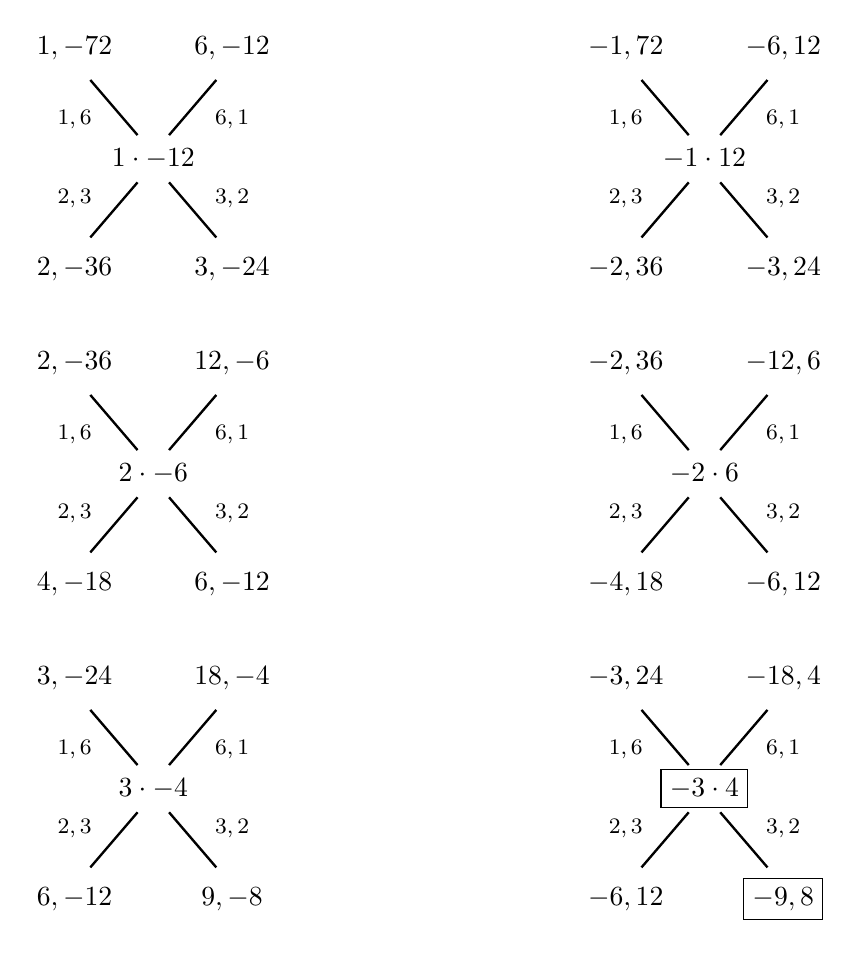
\begin{tikzpicture}
	\node at (0,0) {$1 \cdot -12$};

	\node at (-1,0.5) {\footnotesize$1, 6$};
	\draw[line width=0.03cm,label={1}] (-0.2,0.3) -- (-0.8,1);
	\node at (-1,1.4) {$1, -72$};

	\node at (1,0.5) {\footnotesize$6, 1$};
	\draw[line width=0.03cm,label={1}] (0.2,0.3) -- (0.8,1);
	\node at (1,1.4) {$6, -12$};	
	
	\node at (-1,-0.5) {\footnotesize$2, 3$};
	\draw[line width=0.03cm,label={1}] (-0.2,-0.3) -- (-0.8,-1);
	\node at (-1,-1.4) {$2, -36$};

	\node at (1,-0.5) {\footnotesize$3, 2$};
	\draw[line width=0.03cm,label={1}] (0.2,-0.3) -- (0.8,-1);
	\node at (1,-1.4) {$3, -24$};

	\tikzset{shift={(7,0)}}
	
	\node at (0,0) {$-1 \cdot 12$};

	\node at (-1,0.5) {\footnotesize$1, 6$};
	\draw[line width=0.03cm,label={1}] (-0.2,0.3) -- (-0.8,1);
	\node at (-1,1.4) {$-1, 72$};

	\node at (1,0.5) {\footnotesize$6, 1$};
	\draw[line width=0.03cm,label={1}] (0.2,0.3) -- (0.8,1);
	\node at (1,1.4) {$-6, 12$};	
	
	\node at (-1,-0.5) {\footnotesize$2, 3$};
	\draw[line width=0.03cm,label={1}] (-0.2,-0.3) -- (-0.8,-1);
	\node at (-1,-1.4) {$-2, 36$};

	\node at (1,-0.5) {\footnotesize$3, 2$};
	\draw[line width=0.03cm,label={1}] (0.2,-0.3) -- (0.8,-1);
	\node at (1,-1.4) {$-3, 24$};
		
	\tikzset{shift={(-7,-4)}}
	
	\node at (0,0) {$2 \cdot -6$};

	\node at (-1,0.5) {\footnotesize$1, 6$};
	\draw[line width=0.03cm,label={1}] (-0.2,0.3) -- (-0.8,1);
	\node at (-1,1.4) {$2, -36$};

	\node at (1,0.5) {\footnotesize$6, 1$};
	\draw[line width=0.03cm,label={1}] (0.2,0.3) -- (0.8,1);
	\node at (1,1.4) {$12, -6$};	
	
	\node at (-1,-0.5) {\footnotesize$2, 3$};
	\draw[line width=0.03cm,label={1}] (-0.2,-0.3) -- (-0.8,-1);
	\node at (-1,-1.4) {$4, -18$};

	\node at (1,-0.5) {\footnotesize$3, 2$};
	\draw[line width=0.03cm,label={1}] (0.2,-0.3) -- (0.8,-1);
	\node at (1,-1.4) {$6, -12$};
	
	\tikzset{shift={(7,0)}}
	
	\node at (0,0) {$-2 \cdot 6$};

	\node at (-1,0.5) {\footnotesize$1, 6$};
	\draw[line width=0.03cm,label={1}] (-0.2,0.3) -- (-0.8,1);
	\node at (-1,1.4) {$-2, 36$};

	\node at (1,0.5) {\footnotesize$6, 1$};
	\draw[line width=0.03cm,label={1}] (0.2,0.3) -- (0.8,1);
	\node at (1,1.4) {$-12, 6$};	
	
	\node at (-1,-0.5) {\footnotesize$2, 3$};
	\draw[line width=0.03cm,label={1}] (-0.2,-0.3) -- (-0.8,-1);
	\node at (-1,-1.4) {$-4, 18$};

	\node at (1,-0.5) {\footnotesize$3, 2$};
	\draw[line width=0.03cm,label={1}] (0.2,-0.3) -- (0.8,-1);
	\node at (1,-1.4) {$-6, 12$};	
	
	\tikzset{shift={(-7,-4)}}
	
	\node at (0,0) {$3 \cdot -4$};

	\node at (-1,0.5) {\footnotesize$1, 6$};
	\draw[line width=0.03cm,label={1}] (-0.2,0.3) -- (-0.8,1);
	\node at (-1,1.4) {$3, -24$};

	\node at (1,0.5) {\footnotesize$6, 1$};
	\draw[line width=0.03cm,label={1}] (0.2,0.3) -- (0.8,1);
	\node at (1,1.4) {$18, -4$};	
	
	\node at (-1,-0.5) {\footnotesize$2, 3$};
	\draw[line width=0.03cm,label={1}] (-0.2,-0.3) -- (-0.8,-1);
	\node at (-1,-1.4) {$6, -12$};

	\node at (1,-0.5) {\footnotesize$3, 2$};
	\draw[line width=0.03cm,label={1}] (0.2,-0.3) -- (0.8,-1);
	\node at (1,-1.4) {$9, -8$};	

	\tikzset{shift={(7,0)}}
	
	\node at (0,0) {\framebox{$-3 \cdot 4$}};

	\node at (-1,0.5) {\footnotesize$1, 6$};
	\draw[line width=0.03cm,label={1}] (-0.2,0.3) -- (-0.8,1);
	\node at (-1,1.4) {$-3, 24$};

	\node at (1,0.5) {\footnotesize$6, 1$};
	\draw[line width=0.03cm,label={1}] (0.2,0.3) -- (0.8,1);
	\node at (1,1.4) {$-18, 4$};	
	
	\node at (-1,-0.5) {\footnotesize$2, 3$};
	\draw[line width=0.03cm,label={1}] (-0.2,-0.3) -- (-0.8,-1);
	\node at (-1,-1.4) {$-6, 12$};

	\node at (1,-0.5) {\footnotesize$3, 2$};
	\draw[line width=0.03cm,label={1}] (0.2,-0.3) -- (0.8,-1);
	\node at (1,-1.4) {\framebox{$-9, 8$}};		
	\end{tikzpicture}
	\]

Therefore, 
	\[
	6x^2 - x - 12= (3x + 4)(2x - 3)
	\]



\newpage



% Problem 4
\problem{10} Use the discriminant of $f(x)= x^2 - 2x + 5$ to determine whether the quadratic function factors over the integers, reals, or complex numbers. \pspace

\sol We know that $D= b^2 - 4ac$. We have $a= 1$, $b= -2$, and $c= 5$. Therefore,
	\[
	D= b^2 - 4ac= (-2)^2 - 4(1)5= 4 - 20= -16
	\]
Because $D < 0$, we know that $f(x)$ does not factor over the integers or the real numbers. However, $f(x)$ does factor over the complex numbers. In fact, we have\dots
	\[
	f(x)= x^2 - 2x + 5= \big( x - (1 + 2i) \big) \big( x - (1 - 2i) \big) 
	\]


\end{document}